\begin{figure}[t]
	\begin{minipage}[b]{0.49\linewidth}
		\centering
		\centerline{ 
\includegraphics[width=\textwidth]{disp} }
		\centerline{\scriptsize{(a) Estimated disparity map }}\medskip
	\end{minipage}
	\hfill
	\begin{minipage}[b]{0.49\linewidth}
		\centering
		\centerline{
\includegraphics[width=\textwidth]{wmf} }
		\centerline{\scriptsize{(b) Enhanced disparity map}}\medskip
	\end{minipage}
	\begin{minipage}[b]{1\linewidth}
		\centering
		\centerline{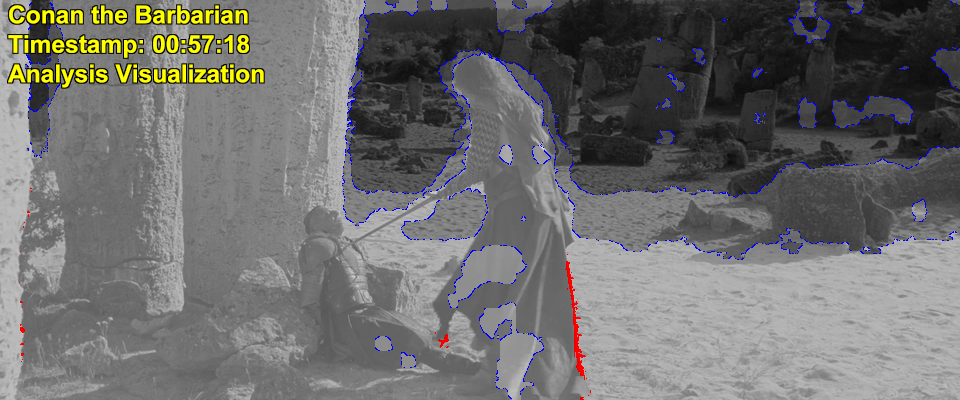
\includegraphics[width=\textwidth]{visualization} }
		\centerline{\scriptsize{(c) Visualization of final result }}
	\end{minipage}
    \caption{Examples of a disparity map before~(a) and after~(b) weighted-median
        filtering. The resulting visualization~(c) that we offer to content
        creators is a disparity map overlaid on the source frame. We use blue to mark
        the disparity edges and red to mark any inconsistencies
        between motion- and disparity-map edges.}
	\label{fig:disp}
\end{figure}
